% !TeX spellcheck = en_US
\chapter{IceAct Parameterization}

The simulation results discussed in chapter \ref{chap:iceact_sim} can now be used to parameterize the telescope response of IceAct. The major goal of this is to provide a fast way to evaluate the detection probability of incident photons in each camera pixel which is done by elaboration of a lookup table (\textit{LUT}). Afterwards, the high computational effort by propagating each Cherenkov photon through the whole \geant model is not needed any more. To achieve this, one needs a well-defined strategy to convert the simulated raw data into a meaningful parameterization. 

\section{Parameterization Strategy}\label{sec:param:strategy}

The following sections discuss the step-by-step strategy to get \textit{detection efficiency maps} out of the \geant data. These maps will describe the direction-dependent detection probabilty for a certain wavelength range and a certain camera pixel.

\subsection{Kernel Density Estimation (KDE)}

\textit{Kernel density estimation} (\textit{KDE}) is a non-parametric\footnote{A non-parametric method names a statistical approach based on a non-defined model that is deduced directly from data.} method to estimate a probability density function of a random variable by a given finite data sample. The standard \textit{kernel density estimator}
\begin{align}
	\hat{f}(x)=\frac{1}{nh}\sum_{i=1}^{n}K\left(\frac{x-X_i}{h}\right)\,,
	\label{eq:kde}
\end{align}
is the sum of \textit{kernel functions} $K(\dots)$ for each data point $X_i$. The non-negative parameter $h$ is the \textit{bandwidth} and is a measure for the smoothing of the resulting KDE: the KDE gets smoother with increasing $h$. Due to the normalization factor, $\hat{f}(x)$ is normed to
\begin{align}
	\int\limits_{-\infty}^{+\infty}\hat{f}(x)dx \equiv 1\,.
	\label{kde:norm}
\end{align}

\begin{figure}[h]
	\centering
	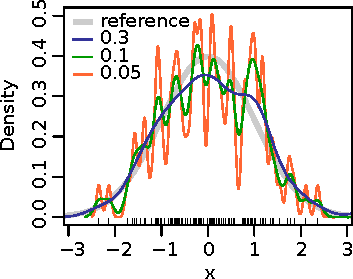
\includegraphics[width=0.5\textwidth]{KDE_example.pdf}
	\caption[Example KDE with different smoothing]{\textbf{Example KDE with different smoothing.} \cite{kde:example_plot} Kernel density estimation is applied on a data sample with 100 random numbers drawn from a normal distribution (gray curve). The blue, green, and orange curves have different bandwidths.}
	\label{kde:example_1d}	
\end{figure}

The kernel function can be a very distinct function that can in principle describe any probability density. In this parameterization method a Gaussian kernel
\begin{align}
	K(t) = \frac{1}{\sqrt{2\pi}}e^{-\frac{1}{2}t^2}
\end{align}
is used.

In order to get the KDE describing the probability density appropriately, one has to choose a reasonable bandwith for the given data sample size. As shown in figure \ref{kde:example_1d}, too low bandwith results in a spiky, fluctuating KDE. If the bandwidth is too high, one might get a rather inaccurate estimator. Therefore it seems reasonable to choose different bandwidth in regions with different amount of statistics which then is called \textit{adaptive} kernel density estimation. \cite{kde:schoenen, kde:wangwang}

\subsubsection{Adaptive KDE with Gaussian Kernel}
As one can see in the simulation results (cf. \todo{verweis zu map}) and in figure \ref{kde:example_scatter}, each pixel has a certain region of photon directions where it is efficient. However, each pixel is almost \enquote{blind} for most other directions. This results in statistically stable -- \enquote{dense} -- regions but also \enquote{sparse} regions dominated by scattered photons that undergo large statistical fluctuations. Thus, and based on the former conclusions, an approach to adapt the bandwidth to the local statistics should perform well. In this thesis, an algorithm presented by \textsc{B. Wang} and \textsc{X. Wang} in \cite{kde:wangwang} which has been implemented within the scope of \cite{kde:schoenen} is used. The adaptive (in principle weighted) kernel density estimator is calculated by \cite{kde:schoenen,kde:wangwang}
\begin{align}
	f(\vec{x}) = \sum_{i=1}^{n} \frac{w_i}{N_i}e^{-\frac{1}{2}(\vec{x}-\vec{X_i})^T \frac{1}{h\lambda_i} \mathbf{C}^{-1} (\vec{x}-\vec{X_i})}\,,
\end{align}
with
\begin{vardescription}
	n & total number of data points,\\
	w_i & weight of th $i$-th data point,\\
	N_i & Gaussian normalization,\\
	\vec{X_i} & coordinate vector of the $i$-the data point,\\
	h & global bandwidth factor,\\
	\lambda_i & local bandwidth factor,\\
	\mathbf{C} & covariance matrix.\\
\end{vardescription}
The global bandwidth factor $h$ is calculated by the \textit{Silverman rule} \cite{kde:schoenen,kde:wangwang}
\begin{align}
	h = \left(\frac{n(d+2)}{4}\right)^{-\frac{1}{d+4}}\,,
\end{align}
where $d$ equals the number of dimensions of the data (here $d=2$). The local bandwidth $\lambda_i$ is the factor where the local statistics of each data point comes in. It is defined as \cite{kde:schoenen,kde:wangwang}
\begin{align}
	\lambda_i = \left(\frac{\hat{f}(\vec{X_i})}{g}\right)^{-\alpha}\,,
\end{align}
with
\begin{vardescription}
	\hat{f}(\vec{X_i}) = f(\vec{X_i})|_{w_i=\lambda_i=1}\,,\\
	\ln{g} = n^{-1} \sum_{i=1}^{n} \ln{\hat{f}(\vec{X_i})}\,,\\
	\alpha\in[0,1]\,.
\end{vardescription}
For the IceAct parameterization the sensitivity parameter $\alpha$ is set to $\alpha=\num{0.3}$, since this has been shown to be an appropriate value as well as in \cite{kde:schoenen}. Additionally, all $n$ photon hits have the same weight, which results in \cite{kde:schoenen,kde:wangwang}
\begin{align}
	w_i = \frac{1}{n}\,.
\end{align}

\subsubsection{Bootstrapping}

One problem of kernel density estimation is that it does not provide any statistical information, i.e. \enquote{how precise} the probability density is estimated. Since the data set used for the KDE is just a random sample of the underlying \textit{probability density function} (\textit{PDF}), one needs a method to draw multiple subsamples from the given data which is known as \textit{resampling}.

More specifically, the \textit{bootstrapping} method is used. It is type of resampling where $n$ data points are drawn from $n$ data points with replacement, so that one data point can possibly be chosen multiple times or not at all. The probability of drawing a point is equal for all points given by $\frac{1}{n}$. Hence, the probability of a not drawing a single data point in a bootstrapped sample is
\begin{align}
	\left(1-\frac{1}{n}\right)^n \overset{n\to\infty}{\longrightarrow} \approx\SI{37}{\percent}\,.
\end{align}
For a large sample size $n\to\infty$ this means that $1-\left(1-\frac{1}{n}\right)^n\approx\SI{63}{\percent}$ of the data points in a bootstrapped data sample are statistically independent.

The bootstrapping can now be repeated $k$ times and for each subsample $\{\vec{X}_i^\ast\}$ an adaptive KDE is done resulting in $k$ KDE functions $f_{\{\vec{X}_i^\ast\}}(\vec{x})$. The final KDE function $f(\vec{x})$ and its uncertainty is then given by the mean and the standard deviation,~\cite{kde:bootstrapping,kde:schoenen}
\begin{subequations}
	\begin{align}
		f(\vec{x}) &= \frac{1}{k}\sum_{i=1}^{k} f_{\{\vec{X}_i^\ast\}}(\vec{x})\\
		\sigma_{f(\vec{x})}	&= \sqrt{\frac{1}{k}\sum_{i=1}^{k}\left(f_{\{\vec{X}_i^\ast\}}(\vec{x}) - f(\vec{x})\right)^2}
	\end{align}
\end{subequations}

\subsection{Coordinate Transformation for KDE}

\todo{write}

\subsection{KDE Evaluation}

\todo{write?}

\subsubsection{The HEALPix Algorithm}

In order to account for the spherical shape of the angles of incidence it is useful to have angular bins with equal areas. Therefore, in this parameterization method, the \textit{HEALPix} (\textbf{H}ierarchical \textbf{E}qual \textbf{A}rea iso\textbf{L}atitude \textbf{Pix}elization) algorithm is used. It allows a uniform pixelization of incidence angles to the telescope.\\

\begin{figure}[H]
	\centering
	\saveimageheight[width=0.48\textwidth]{HEALPix_pixelization_steps.png}
	\begin{subfigure}[t]{0.48\textwidth}
		\centering
		\raiseimage[width=\textwidth]{HEALPix_pixelization_standard.pdf}
		\subcaption{Orthographic (top) and cylindrical (bottom) view of the pixelization scheme at the initial step ($k=0$). The sphere is tessellated into 12 quadrilateral equal-area panes with $N_\theta=3$ divisions in zenith and $N_\phi=4$ divisions in azimuth angle. }
		\label{}
	\end{subfigure}
	\hfill
	\begin{subfigure}[t]{0.48\textwidth}
		\centering
		\usebox{\savedimage}
		\subcaption{Further subdivision steps starting with the initial base resolution $k=0$ (top left) and $k=1,2,3$ clockwise. The light gray shaded area marks one of the 8 identical polar base-resolution pixels while the dark light shaded area marks one of the 4 identical equatorial base-resolution pixels.}
		\label{}
	\end{subfigure}
	\caption[Pixelization scheme of the HEALPix algorithm]{\textbf{Pixelization scheme of the HEALPix algorithm.} \cite[adapted]{healpix:paper}}
	\label{healpix:pixelization}
\end{figure}

The basic idea is to subdivide the sphere into 12 quadrilateral equal-area panes which can then further divided uniformly into more sub panes as shown in figure \ref{healpix:pixelization}. A parameter $k$ numbers the subdivision step starting with the base resolution at $k=0$ so that the number of sub panes per each of the 12 panes is $N_{\text{side}}^2=\left(2^k\right)^2$. Hence, the total amount of pixels on the sphere is then \cite{healpix:paper}
\begin{align}
N_\text{pix} = 12N_\text{side}^2\,.
\label{eq:npix}
\end{align}

The angular resolution $\theta_\text{pix}$ is defined to be the square root of the angular area $\Omega_\text{pix}$. Descriptively, it is the angular length of a pixel edge. $\Omega_\text{pix}$ in turn can be calculated by dividing the total angular area of a sphere $4\pi$ by the total number of pixels $N_\text{pix}$, which yields \cite{healpix:paper}
\begin{align}
	\theta_\text{pix} = \sqrt{\Omega_\text{pix}} = \sqrt{\frac{4\pi}{N_\text{pix}}} \overset{\eqref{eq:npix}}{=} \sqrt{\frac{4\pi}{12N_\text{side}^2}} = \sqrt{\frac{\pi}{3}}N_\text{side}^{-1}\,[\si{\radian}]\,.
\end{align} 

\begin{table}[h]
\centering
\begin{tabular}{S[table-format=2.0]|S[table-format=4.0]|S[table-format=9.0]|S[table-format=2.2]}
\multicolumn{1}{l|}{$k$} & \multicolumn{1}{l|}{$N_\text{side} = 2^k$} & \multicolumn{1}{l|}{$N_\text{pix} = 12N_\text{side}^2$} & \multicolumn{1}{l}{$	\theta_\text{pix} = \sqrt{\Omega_\text{pix}}$} \\
\hline
0  & 1    & 12        &  \SI{58.6}{\degree}\\
1  & 2    & 48        &  \SI{29.3}{\degree}\\
2  & 4    & 192       &  \SI{14.7}{\degree}\\
3  & 8    & 768 	  &  \SI{7.33}{\degree}\\
4  & 16   & 3072      &  \SI{3.66}{\degree}\\
5  & 32   & 12288     &  \SI{1.83}{\degree}\\
6  & 64   & 49152     &  \SI{55.0}{\arcminute}\\
7  & 128  & 196608    &  \SI{27.5}{\arcminute}\\
8  & 256  & 786432    &  \SI{13.7}{\arcminute}\\
9  & 512  & 3145728   &  \SI{6.87}{\arcminute}\\
10 & 1024 & 12582912  &  \SI{3.44}{\arcminute}\\
11 & 2048 & 50331648  &  \SI{1.72}{\arcminute}\\
12 & 4096 & 201326592 &  \SI{51.5}{\arcsecond}\\
13 & 8192 & 805306368 &  \SI{25.8}{\arcsecond}\\
\multicolumn{1}{c|}{\vdots} & \multicolumn{1}{c|}{\vdots} & \multicolumn{1}{c|}{\vdots} & \multicolumn{1}{c}{\vdots} \\
\end{tabular}
\caption[HEALPix parameters and resulting angular resolutions]{\textbf{HEALPix parameters and resulting angular resolutions.} $k$ represents the number of dividing iterations on the 12 panes, $N_\text{side}$ the number of tiles per pane edge, $N_\text{pix}$ the total number of pixels, and $\theta_\text{pix}$ the angular resolution defined by the angular length of a pixel edge. \cite{healpix:paper}}
\end{table}

For the application in this simulation the pixelization of a whole sphere is not needed since the telescope only has a field of view of about \SI{12}{\degree} (i.e. $\theta \leq \SI{6}{\degree}$). Considering that, one only needs a smaller sector of pixels around the zenith at $\theta = \SI{0}{\degree}$ which reduces the number of needed HEALPix to a factor of
\begin{align}
	\Gamma = \frac{1}{4\pi}\int\limits_{0}^{2\pi}\int\limits_{0}^{\theta_\text{max}}\sin{\theta} d\theta d\phi = \frac{1-\cos\theta_\text{max}}{2}\,.
	\label{eq:spherefactor}
\end{align}
For the IceAct simulation with $\theta_\text{max} = \SI{10}{\degree}$ this leads to only about \SI{0.76}{\percent} of the sphere needed to be pixelized.

An additional important supplement is that the HEALPix numbering scheme is hierarchical. The standard numbering scheme -- called \enquote{ring scheme} -- starts at the zenith $\theta = \SI{0}{\degree}$ and follows a spiral for increasing zenith angles. There are two advantages of this numbering scheme for the use case of IceAct simulation. On the one hand, the unambiguous numbering makes it unnecessary for the directional coordinates $(\theta, \phi)$ to be saved, but only the ordinal number $i_\text{HP}$. In order to reconstruct the direction in polar coordinates, one only has to know the pixelization parameter $N_\text{nside}$. On the other hand, the ring scheme and the fact that the simulated directions are limited by $\theta_\text{max}$ result in a distinct maximum ordinal number $i_\text{HP}^\text{max}$ and one can just ignore all pixels beyond this number. This allows to save information very efficiently by using HEALPixes. 

\subsubsection{KDE Renormalizaion: Detection Efficiency}

By using the adaptive KDE method one gets a probability density function which implies normalization (cf. equation \eqref{kde:norm}). In order to get to an actual efficiency, one has to do a renormalization.

The ansatz is made by describing the differential detection efficiency of the $i$-th SiPM in the angular area $d\Omega$ as a ratio of \textit{detection density} in the $i$-th SiPM $\rho_{\text{det},i,\Delta\lambda}(\theta,\phi)$ and \textit{simulation density} $\rho_{\text{sim},\Delta\lambda}(\theta,\phi)$ for each wavelength range $\Delta\lambda$ by
\begin{align}
\frac{d\epsilon_{i,\Delta\lambda}}{d\Omega}(\theta,\phi) = \frac{1}{d\Omega} \frac{\rho_{\text{det},i,\Delta\lambda}(\theta,\phi)}{\rho_{\text{sim},\Delta\lambda}(\theta,\phi)}\,,
\end{align}

Hereafter, the densities are derived by asking following questions.

\minisec{How many photons are detected in SiPM $i$ and wavelength range $\Delta\lambda$?} 
Follows directly from the amount of data points used for KDE. $\rightarrow~N_{\text{det},i,\Delta\lambda}$

\minisec{How many photons are simulated in the wavelength range $\Delta\lambda$?}
Obviously needed to make a statement on the ratio of detected photons. $\rightarrow N_{\text{sim},\Delta\lambda}$\\
The ratio of detected and simulated photons in the $i$-th SiPM and the wavelength range~$\Delta\lambda$ can then be defined as the average detection efficiency 
\begin{align}
	\bar{\epsilon}_{i,\Delta\lambda} = \frac{N_{\text{det},i,\Delta\lambda}}{N_{\text{sim},\Delta\lambda}}\,.
\end{align}

\minisec{What is the maximum simulated zenith angle?}
Needed to calculate the ratio $\Gamma$ of the total spherical area that is evaluated (cf. equation~\eqref{eq:spherefactor}). For the IceAct simulation this is $\theta_\text{max} = \SI{10}{\degree}$. $\rightarrow \theta_\text{max}$

\minisec{What size does the angular area have which the KDE is evaluated for?}
This is caused by the evaluation of a continuous PDF at discrete points. To do so, one has to consider the angular area $\Omega_\text{HP}$ a discrete value is set to be constant for. Thanks to the use of HEALPixes, the angular area of all pixels is constant and follows from the resolution parameter $N_\text{side}$ by
\begin{align}
	\Omega_\text{HP} = \frac{4\pi}{N_\text{pix}} \overset{\eqref{eq:npix}}{=} \frac{\pi}{3N_\text{side}^2}\,.
	\label{eq:omega_hp}
\end{align}

From the former considerations one can conclude the densities given by
\begin{subequations}
	\begin{align}
		\rho_{\text{det},i,\Delta\lambda}(\theta,\phi) &= 
		\begin{cases}
			N_{\text{det},i,\Delta\lambda}\cdot KDE_{i,\Delta\lambda}(\theta,\phi) & ,\,\theta\leq\theta_\text{max}\\
			0 & ,\, \theta > \theta_\text{max}
		\end{cases}\,,
		\label{eq:rho_det}
		\\
		\rho_{\text{sim},\Delta\lambda}(\theta,\phi) &= 
		\begin{cases}
			\frac{N_{\text{sim},\Delta\lambda}}{4\pi\Gamma} & ,\,\theta\leq\theta_\text{max}\\
			0 & ,\, \theta > \theta_\text{max}
		\end{cases}\,.
		\label{eq:rho_sim}
	\end{align}
\end{subequations}

In equation \eqref{eq:rho_det}, $N_{\text{det},i,\Delta\lambda}$ rescales the KDE to be normed to the total amount of detected photons. The factor $(4\pi\Gamma)^{-1}$ in equation \eqref{eq:rho_sim} takes account of the zenith angle limit in the simulation so that the densities have the \enquote{unit}
\begin{align}
	[\rho] = \frac{\text{particles}}{\text{angular area}}\,.
\end{align}

Additionally, one can exploit the equal area properties of the HEALPixes by evaluating the detection efficiency at the central points of each HEALPix $(\theta^\ast_\text{HP},\phi^\ast_\text{HP})$ and setting this value to be a constant in each HEALPix area. Hence we can calculate the detection efficiency by
\begin{align}
	\epsilon_{i,\Delta\lambda,\text{HP}}(\theta\leq\theta_\text{max}) &= \iint_{\Omega_\text{HP}}  \frac{d\epsilon_{i,\Delta\lambda}}{d\Omega}(\theta^\ast_\text{HP},\phi^\ast_\text{HP}) d\Omega\nonumber\\
	&= \iint_{\Omega_\text{HP}}\frac{1}{d\Omega}\frac{N_{\text{det},i,\Delta\lambda}(\theta^\ast_\text{HP},\phi^\ast_\text{HP})}{N_{\text{sim},\Delta\lambda}}\cdot 4\pi\Gamma\cdot KDE_{i,\Delta\lambda}(\theta^\ast_\text{HP},\phi^\ast_\text{HP})d\Omega\nonumber\\
	&= \frac{N_{\text{det},i,\Delta\lambda,\text{HP}}}{N_{\text{sim},\Delta\lambda}}\cdot 4\pi\Gamma\cdot KDE_{i,\Delta\lambda,\text{HP}}\nonumber\\
	&\overset{\eqref{eq:spherefactor}}{=} \frac{N_{\text{det},i,\Delta\lambda,\text{HP}}}{N_{\text{sim},\Delta\lambda}}\cdot 2\pi(1-\cos\theta_\text{max})\cdot KDE_{i,\Delta\lambda,\text{HP}}\,,
	\label{eq:deteff}
\end{align}
with $N_{\text{det},i,\Delta\lambda,\text{HP}}\coloneqq N_{\text{det},i,\Delta\lambda}(\theta^\ast_\text{HP},\phi^\ast_\text{HP})$ and $KDE_{i,\Delta\lambda,\text{HP}}\coloneqq KDE_{i,\Delta\lambda}(\theta^\ast_\text{HP},\phi^\ast_\text{HP})$. This yields to a detection efficiency value for each SiPM~$i$, wavelength range~$\Delta\lambda$, and HEALPix~$\text{HP}$.

To visualize the renormalization process, figure~\ref{deteff:1d_example} shows a 1D example.

\begin{figure}[H]
	\centering
	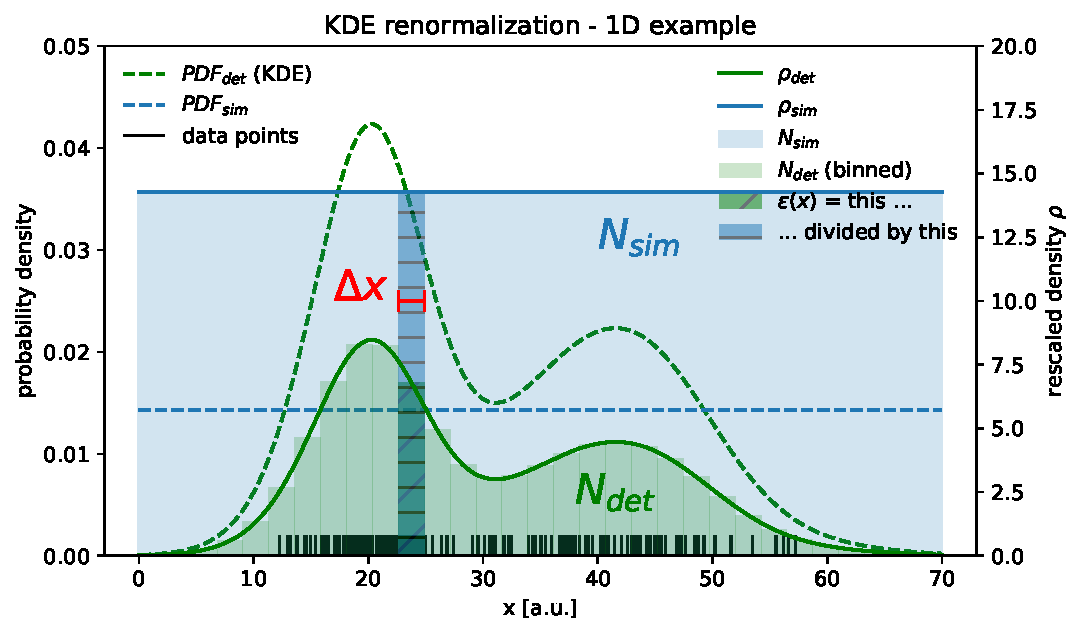
\includegraphics[width=\textwidth]{KDE_renorm_example.pdf}
	\caption[Example: KDE renormalization]{\textbf{Example: KDE renormalization.} 1D example to visualize the renormalization process. In this \enquote{toy simulation} \num{1000}~\enquote{photons} are simulated uniformly in the interval $[\SI{0}{\au},\SI{70}{\au}]$ for which the blue dashed line is the corresponding PDF. \num{200}~\enquote{photons} are detected (black dashes on the $x$ axis) and the PDF is calculated by adaptive kernel density estimation (green dashed line). Since the PDFs are both normalized to $1$ (w.r.t. left $y$ axis), a rescaling is now done (cf. right $y$ axis). The KDE for detected \enquote{photons} is scaled (green solid line) so that the enclosed area is $N_\text{det}=\num{200}$. This is also done with the PDF of simulated data (blue solid line) to correspond to an enclosed area $N_\text{sim}=\num{1000}$. The scaled detection and simulation densities $\rho_\text{det}$ and $\rho_\text{sim}$ are evaluated in bins with size $\Delta x$ which is analogous to the the HEALPix area $\Omega_\text{HP}$ (cf. equation~\eqref{eq:omega_hp}). One gets the detection efficiency $\epsilon(x)$ for each bin by dividing the emphasized hatched areas by each other. The division of areas incorporates the integration over the HEALPix area done in the \enquote{real} evaluation (cf. equation~\eqref{eq:deteff}).}
	\label{deteff:1d_example}	
\end{figure}

\section{Application on Simulated Data}

The parameterization process introduced in section~\ref{sec:param:strategy} can now be applied to the simulation results from \geant. In the following sections, some comparisons and results are shown and discussed.

\subsection{Wavelength Binning}

Since the photon detection efficiency of the SiPMs is a non-constant function of the wavelength (cf. figure~\ref{sipm:pde}), one can optimize the different wavelength ranges or \textit{bin sizes}~$\Delta\lambda$ by equalizing not the bin sizes (\textit{constant binning}) but the detected photons per bin which is further referred to as \textit{adaptive binning}. Figure~\ref{param:wvl_binning} shows a comparison between constant and adaptive wavelength binning.

\begin{figure}[H]
	\centering
	\begin{subfigure}[t]{0.49\textwidth}
		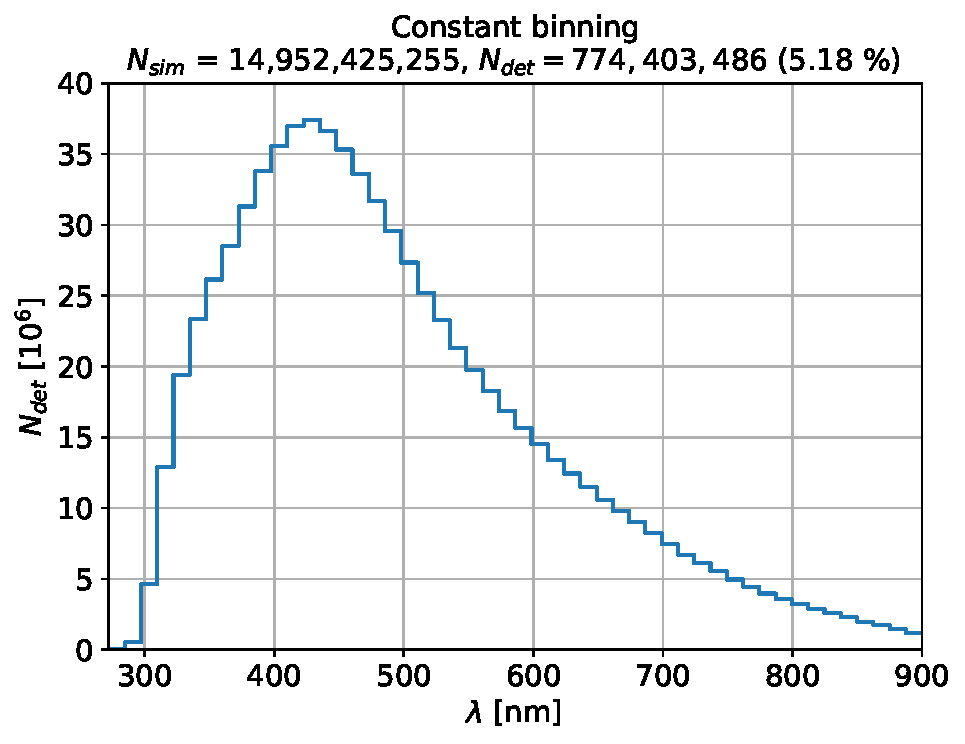
\includegraphics[width=\textwidth]{constant_wvl_bins_hist.pdf}
		\subcaption{constant binning}
		\label{param:wvl_binning:constant}
	\end{subfigure}
	\hfill
	\begin{subfigure}[t]{0.49\textwidth}
		%\includegraphics[width=\textwidth]{wvl_bins_hist.pdf}
		\includegraphics[draft, width=\textwidth]{wvl_bins_hist.pdf}
		\subcaption{adaptive binning}
		\label{param:wvl_binning:adaptive}
	\end{subfigure}
	\caption[Constant vs. adaptive wavelength binning]{\textbf{Constant vs. adaptive wavelength binning.} all wavelengths of photons that are detected by any camera SiPM are histogramized in \num{50} bins between \SI{272}{\nano\meter} and \SI{900}{\nano\meter}. In (\subref{param:wvl_binning:constant}), the \num{50} bins are distributed uniformly in wavelength so that one can see a shape that is quite similar to the PDE of the SiPMs. Figure~(\subref{param:wvl_binning:adaptive}) shows the same data with adaptive bin sizes to equalize the counts per bin. The resulting bin edges are rounded to integer numbers which causes the visible fluctuations.}
	\label{param:wvl_binning}
\end{figure}
\todo{plot mit adaptiven bins}

The adaptive bin edges are calculated by sorting the wavelengths of all simulated particles that are detected by any of the 61 SiPM (i.e. all photons on which the KDE will be applied afterwards (cf. section~\ref{sec:adaptive_vs_nonadaptive})). Next, this sequence is divided into \num{50} parts of equal length. Thus, the wavelengths are divided into consecutive \SI{2}{\percent}-quantiles. In order to get more convenient bin sizes, the quantile limits (or bin edges) are rounded to integer values which obviously result in some fluctuations (cf. figure~\ref{param:wvl_binning:adaptive}).
With the adaptive wavelength binning it is ensured that in each range $\Delta\lambda$ almost the same number of photons is detected which enables a statistically more stable kernel density estimation.

\subsection{Adaptive vs. Non-adaptive KDE}\label{sec:adaptive_vs_nonadaptive}

Now that the wavelength binning is defined, the next step is to take a look on the camera pixels individually. Due to the distinct field of view of each pixel, the direction distribution of each pixel is characteristic. In order to get an idea of the given direction distributions for which the KDE should be calculated, figure \ref{param:example_scatter} shows some exemplary scatter plots of detected photons by an arbitrary camera pixel~$i$ in a wavelength range~$\Delta\lambda$. The need for an adaptive KDE approach is clearly visible by regions with very different statistical densities.

\begin{figure}[H]
	\centering
	\begin{subfigure}[t]{0.49\textwidth}
		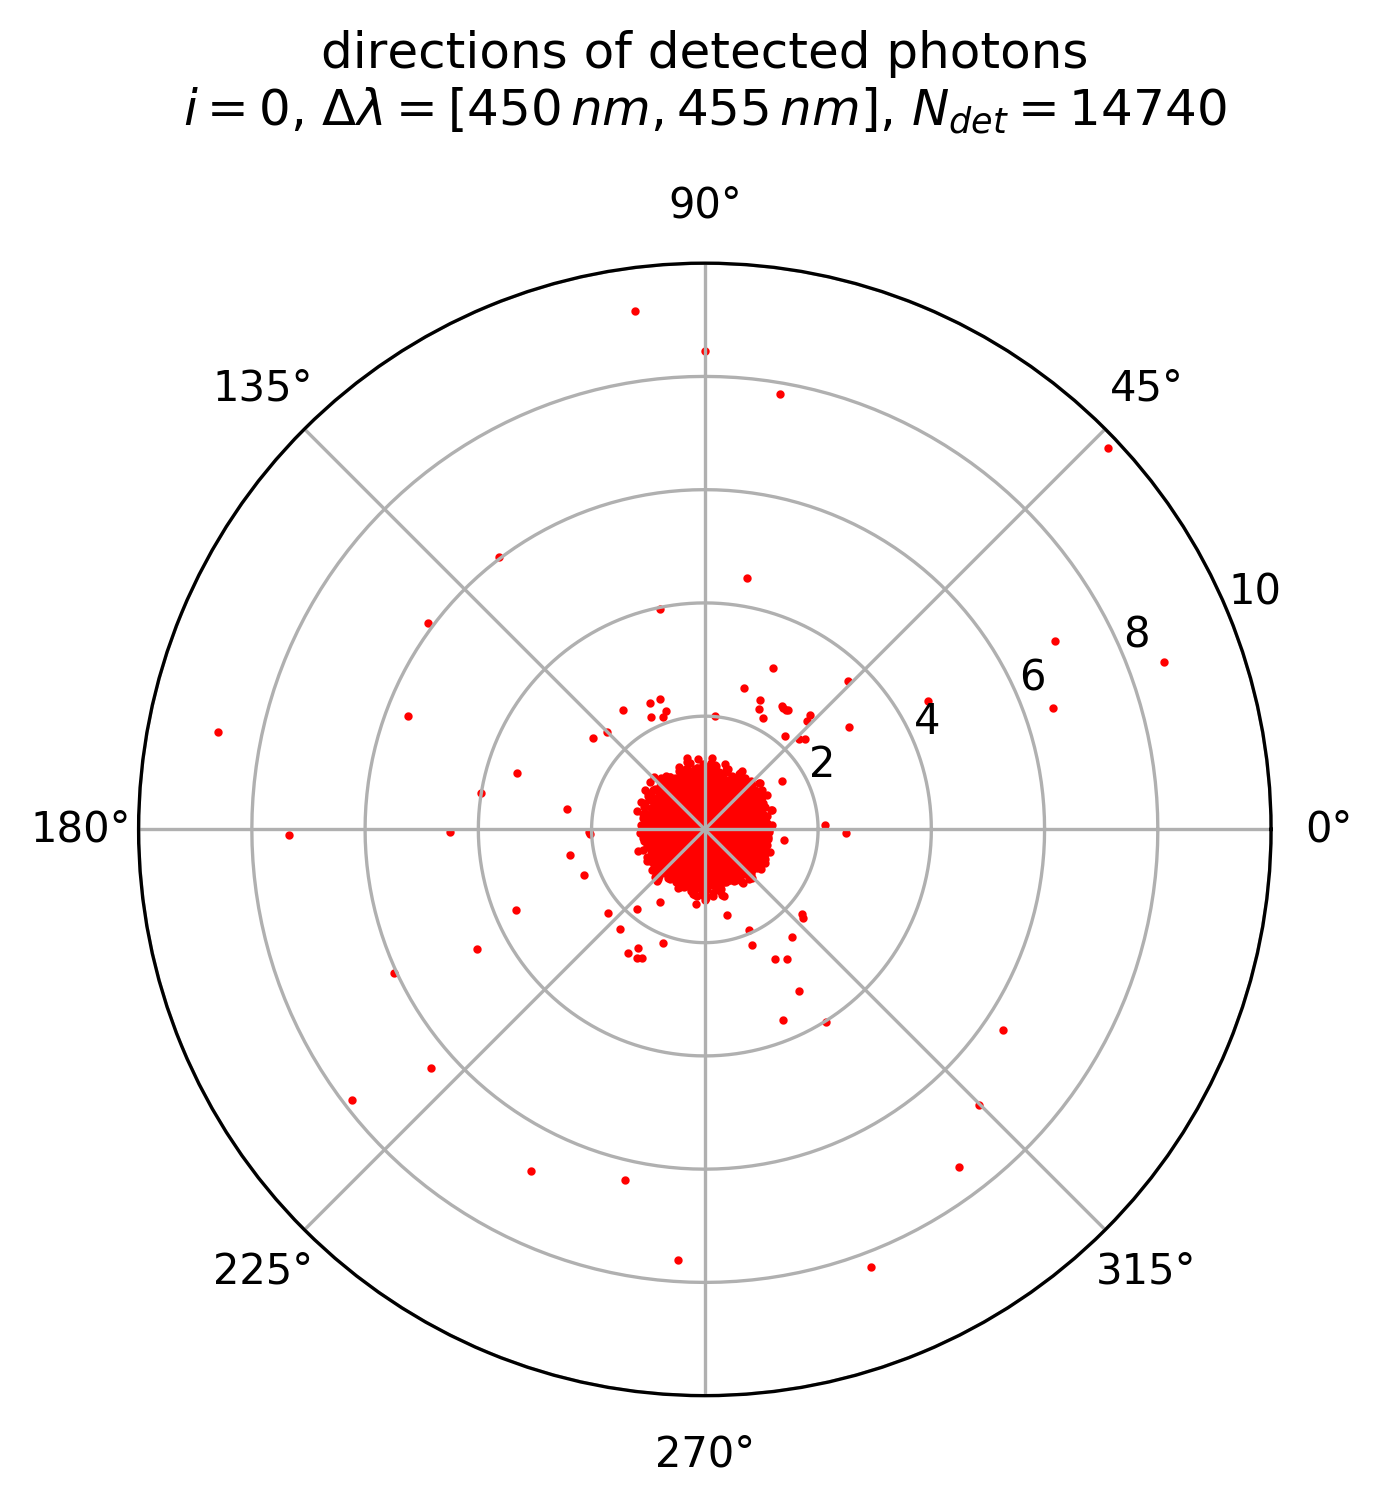
\includegraphics[width=\textwidth]{scatter_px00_wvl450-455nm.png}
		\subcaption{}
		\label{param:example_scatter:1}
	\end{subfigure}
	\hfill
	\begin{subfigure}[t]{0.49\textwidth}
		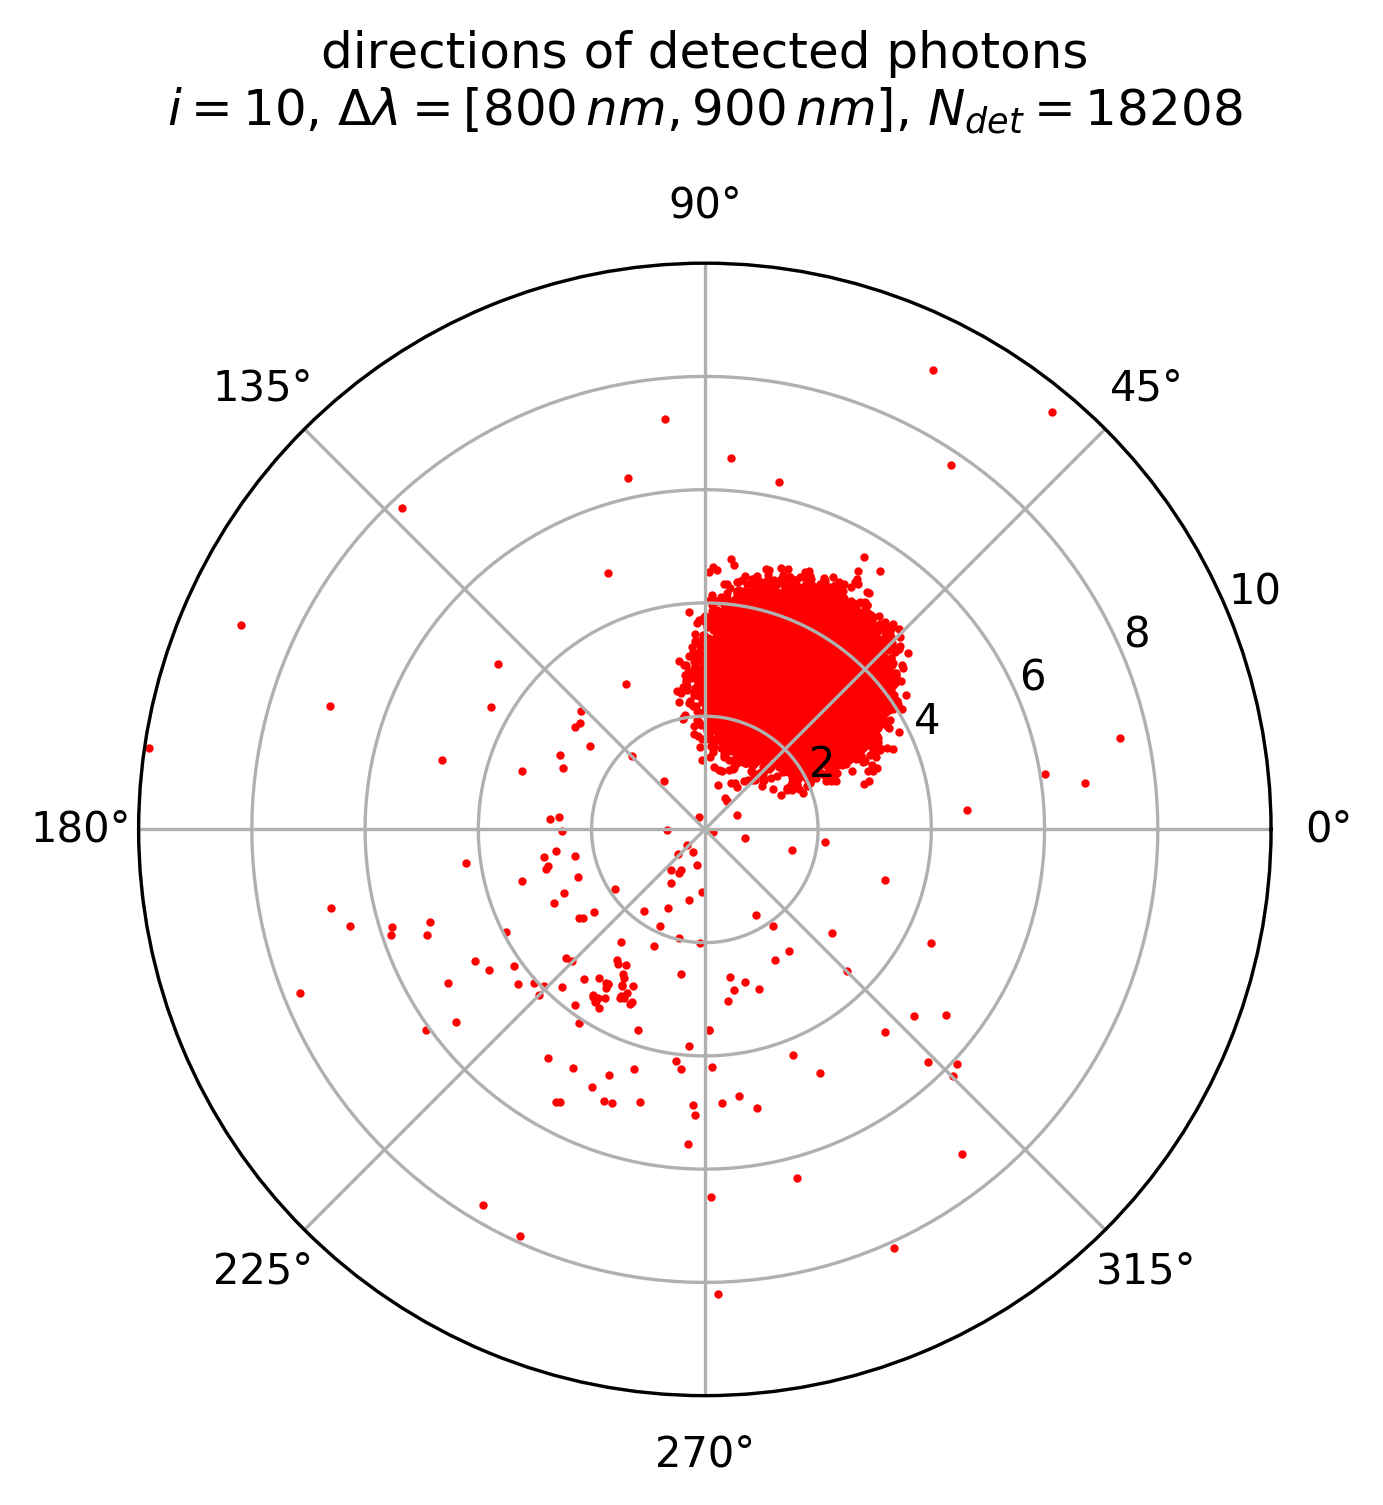
\includegraphics[width=\textwidth]{scatter_px10_wvl800-900nm.png}
		\subcaption{}
		\label{param:example_scatter:2}
	\end{subfigure}
	\vfill
	\begin{subfigure}[b]{0.49\textwidth}
		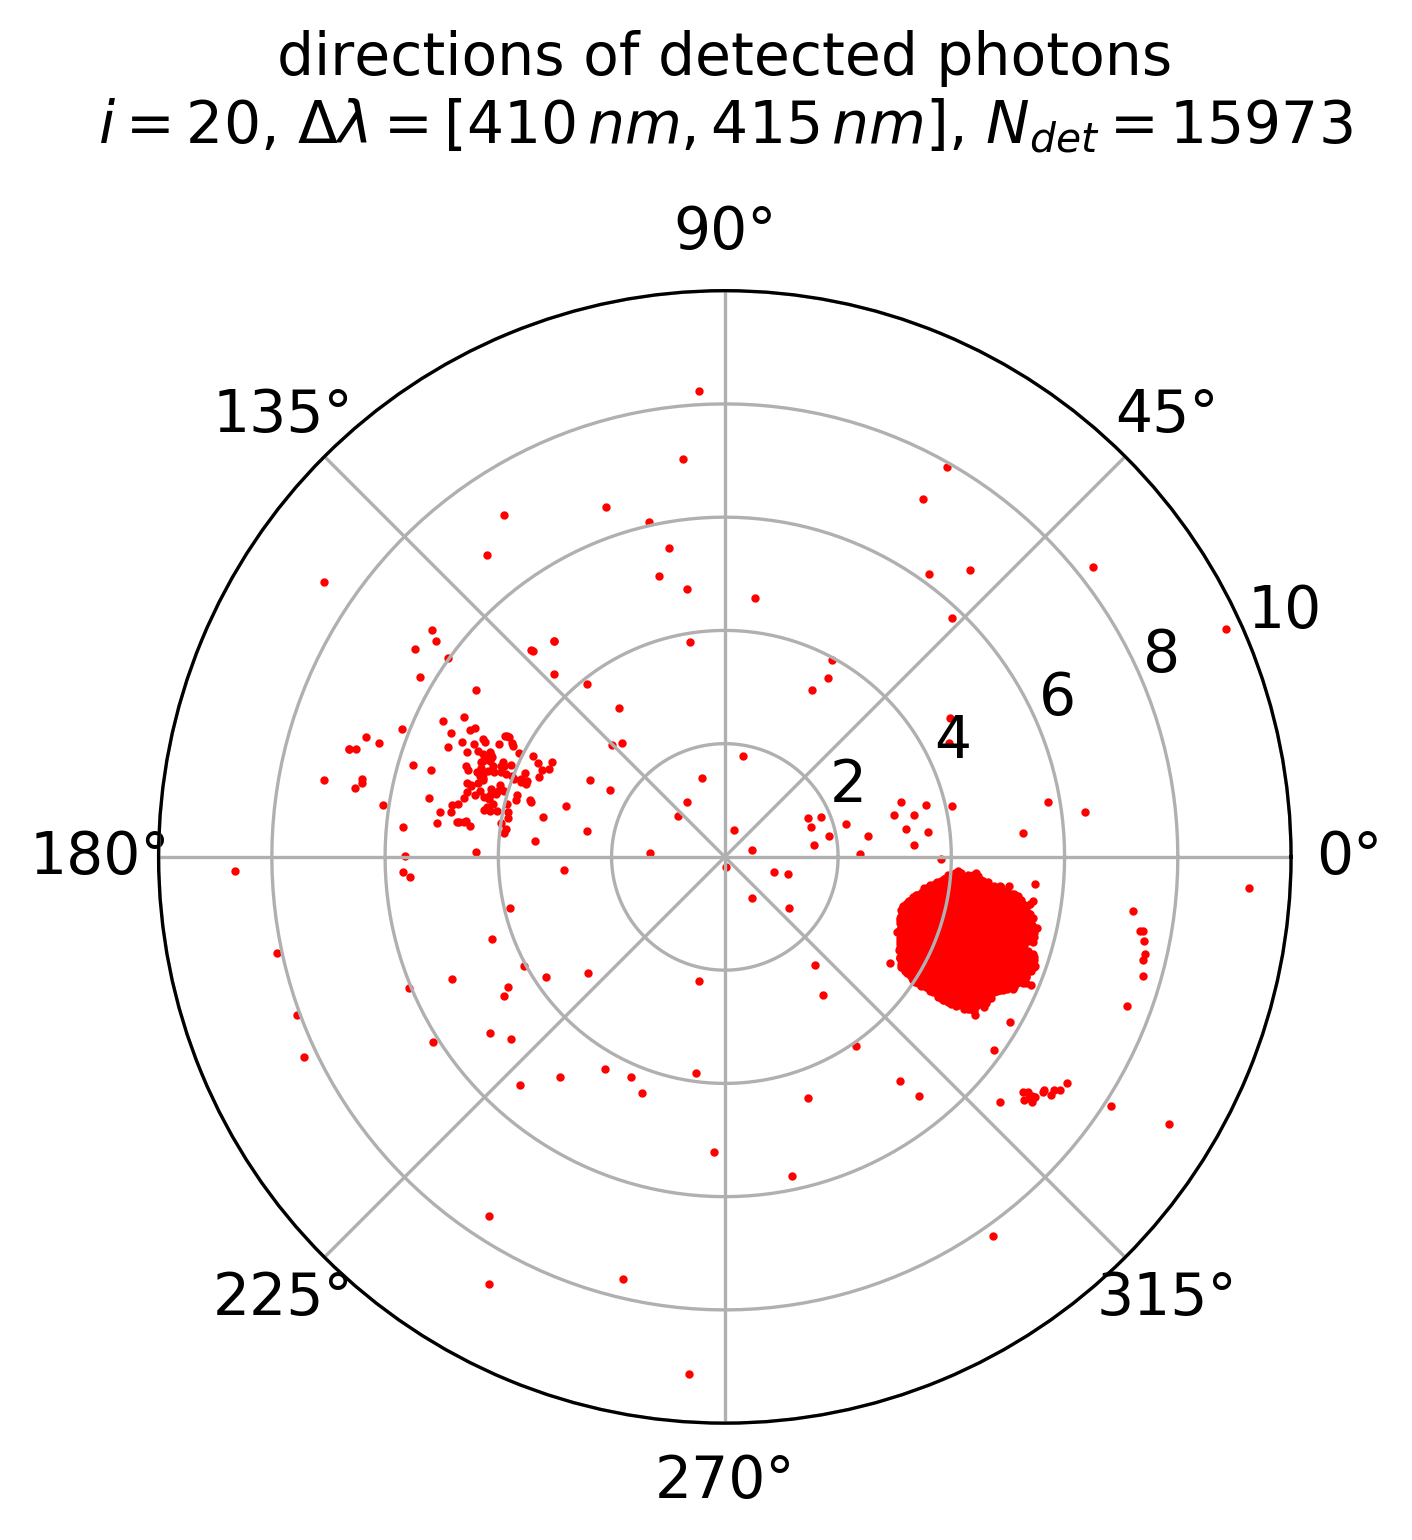
\includegraphics[width=\textwidth]{scatter_px20_wvl410-415nm.png}
		\subcaption{}
		\label{param:example_scatter:3}
	\end{subfigure}
	\hfill
	\begin{subfigure}[b]{0.49\textwidth}
		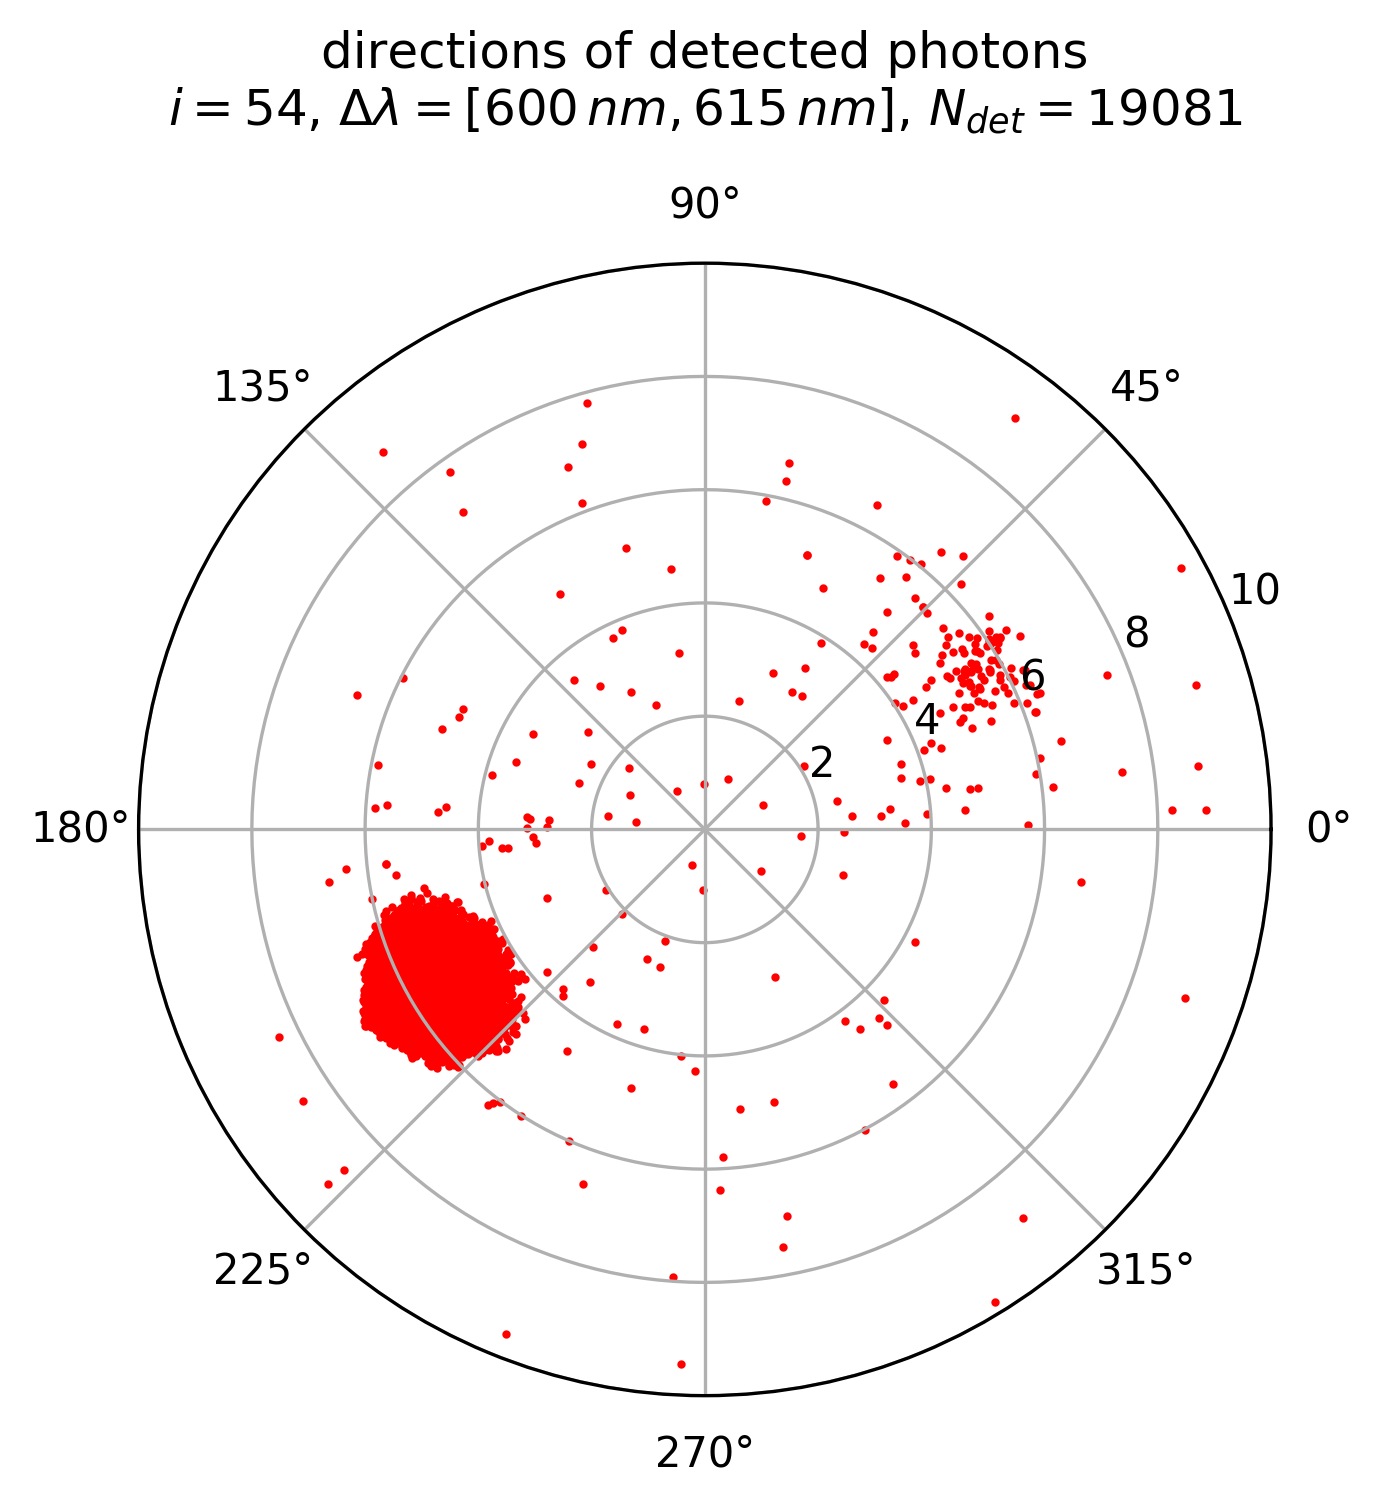
\includegraphics[width=\textwidth]{scatter_px54_wvl600-615nm.png}
		\subcaption{}
		\label{param:example_scatter:4}
	\end{subfigure}
	\caption[Example: directions of detected photons as a scatter plot]{\textbf{Example: directions of detected photons as a scatter plot.} A subset of simulated photon directions that are detected in a given camera pixel $i$ and the wavelength range $\Delta\lambda$ are shown in a polar plot. One can clearly see that there are regions with high and low statistical significance. Additionally, the \textit{ghost image} effect (cf. section~\ref{sec:ghost_image}) is visible in the non-central pixels ((\subref{param:example_scatter:2}), (\subref{param:example_scatter:3}), (\subref{param:example_scatter:4})).}
	\label{param:example_scatter}	
\end{figure}

The regions with very sparse \enquote{dots} can only come from random scattering processes inside the optical system since they are outside the main field of view and the \textit{ghost image} region (cf. section~\ref{sec:ghost_image}). Thus, the probabilty density should be rather constant in these scattering regions. For the KDE, one achieves this by increasing the kernel bandwith. Simultaneously, the \enquote{real} detection regions should be described precisely which is done by reducing the bandwith. The need of an adaptive kernel density approach is given. Figure~\ref{param:kde_comparison} strikingly shows the difference between an adaptive and a non-adaptive KDE. Since the KDEs calculated there are only based on a small subsample of the simulation data, they may give the impression that the adaptive KDE still is very inaccurate in the scattering regions but on the full data sample this is not the case any more by having more scattered photons (cf. section~\ref{sec:deteff_maps}).

\begin{figure}[H]
	\centering
	\begin{subfigure}[t]{0.41\textwidth}
		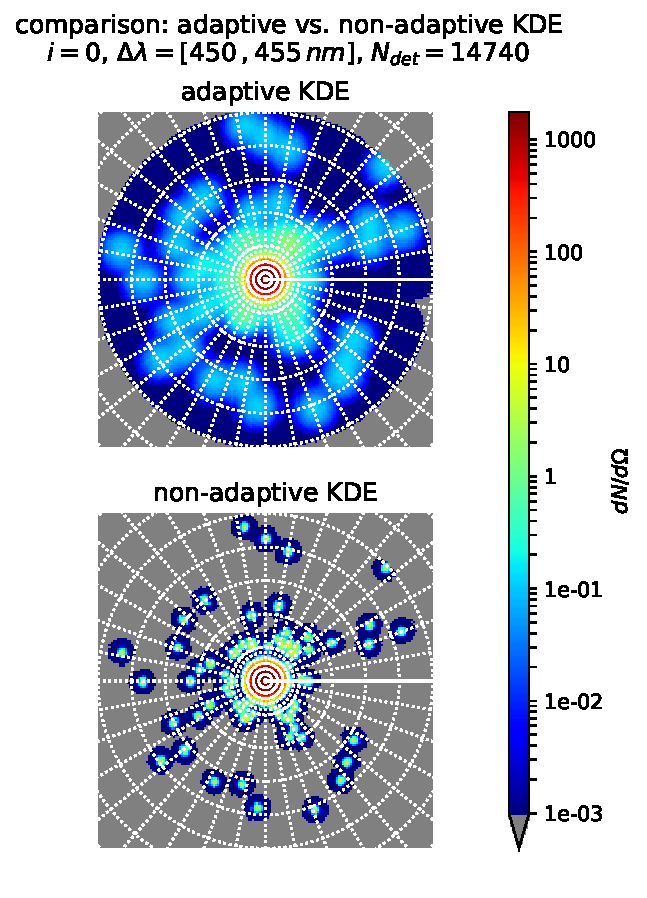
\includegraphics[width=\textwidth]{comparison_adaptive_nonadaptive_px00_wvl450-455.pdf}
		\subcaption{}
		\label{param:kde_comparison:1}
	\end{subfigure}
	\hfill
	\begin{subfigure}[t]{0.41\textwidth}
		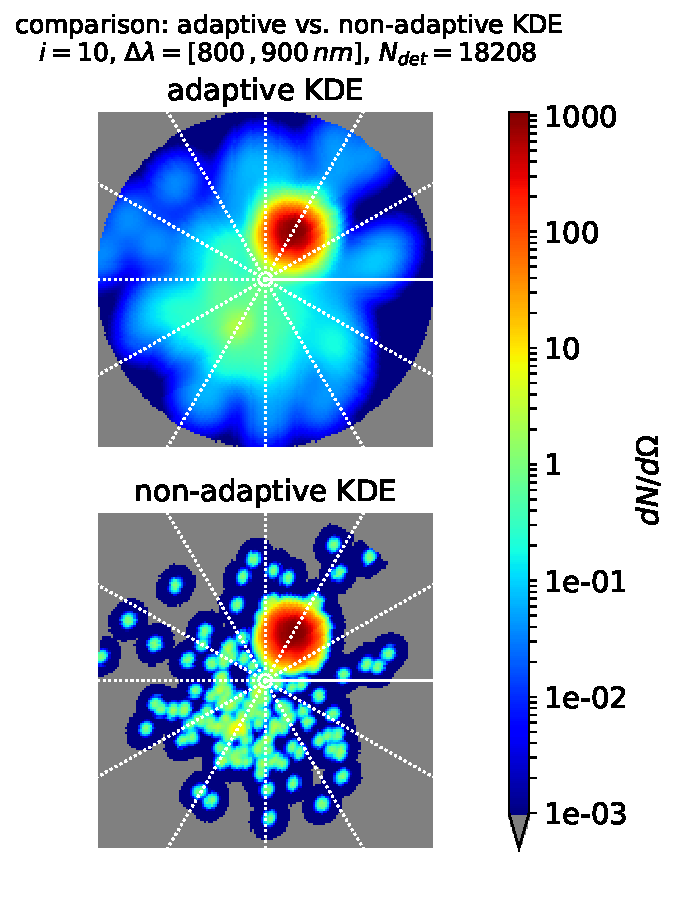
\includegraphics[width=\textwidth]{comparison_adaptive_nonadaptive_px10_wvl800-900.pdf}
		\subcaption{}
		\label{param:kde_comparison:2}
	\end{subfigure}
	\vfill
	\begin{subfigure}[b]{0.41\textwidth}
		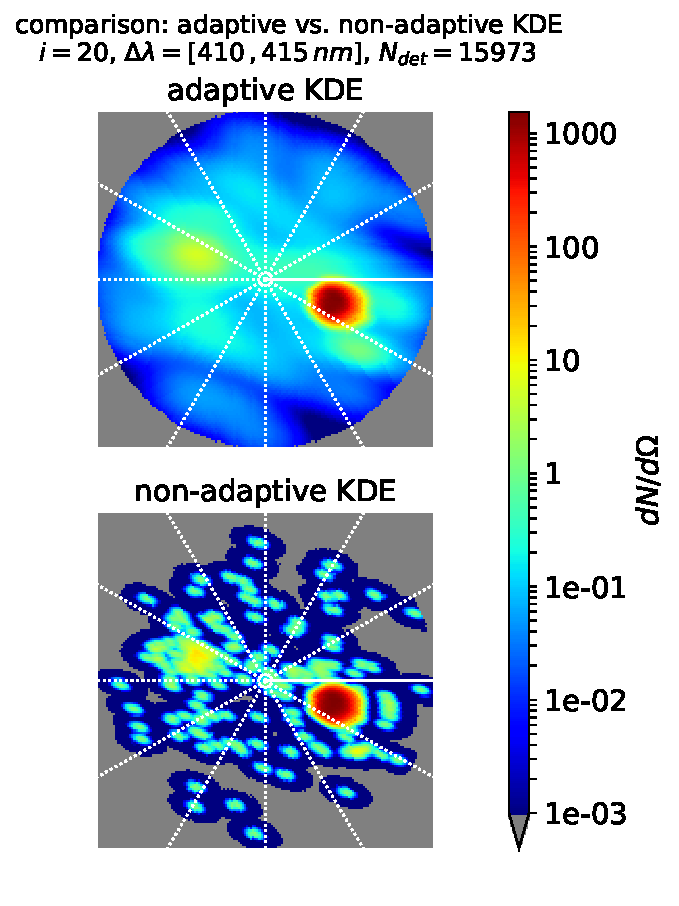
\includegraphics[width=\textwidth]{comparison_adaptive_nonadaptive_px20_wvl410-415.pdf}
		\subcaption{}
		\label{param:kde_comparison:3}
	\end{subfigure}
	\hfill
	\begin{subfigure}[b]{0.41\textwidth}
		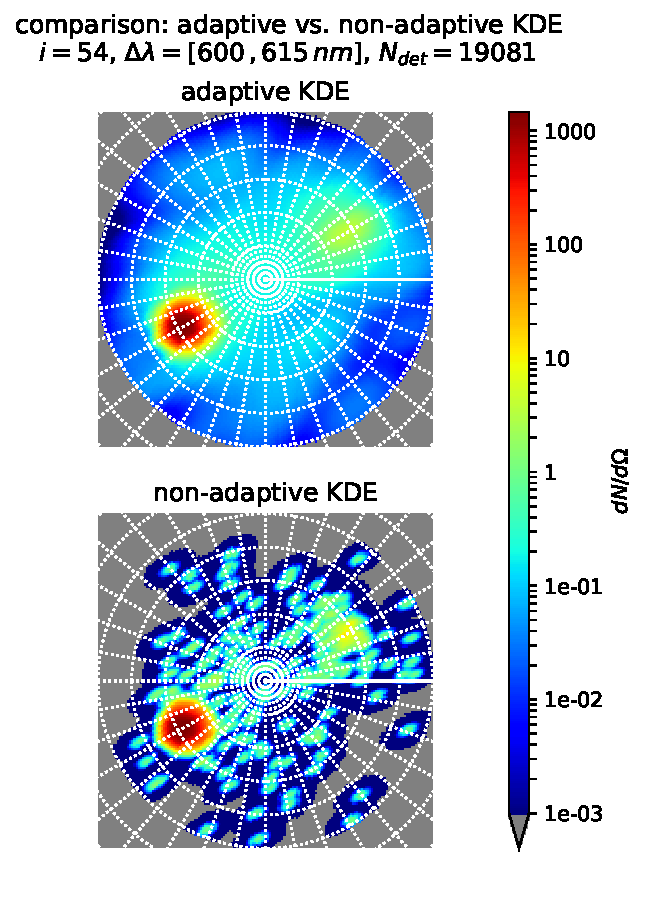
\includegraphics[width=\textwidth]{comparison_adaptive_nonadaptive_px54_wvl600-615.pdf}
		\subcaption{}
		\label{param:kde_comparison:4}
	\end{subfigure}
	\caption[Comparison: adaptive vs. non-adaptive KDE]{\textbf{Comparison: adaptive vs. non-adaptive KDE.} Evaluation of the direction distributions shown in figure~\ref{param:example_scatter} on a HEALPix grid with $N_\text{side}=\num{512}$. The concentric white dashed circles have a zenith distance of $\SI{2}{\degree}$ and the meridians an azimuth distance of $\SI{10}{\degree}$. Differences between an adaptive (top) and non-adaptive (bottom) KDE approach are visible. Especially in the region with low statistics (scattering region), the non-adaptive KDE is dominated by the fluctuations while adaptive KDE blurres the probability density more strongly.}
	\label{param:kde_comparison}		
\end{figure}


\subsection{Detection Efficiency Maps}\label{sec:deteff_maps}

\section{Lookup Table Production}

\section{Application on CORSIKA Air Showers Events}
